\documentclass{article}
\usepackage[utf8]{inputenc}
\usepackage{amsmath}
\usepackage{amssymb}
\usepackage{graphicx}
\graphicspath{{figures/}}
\usepackage{float}
\usepackage{hyperref}
\usepackage{geometry}
\geometry{a4paper, margin=1in}

\title{MPC Mini-Project Final Report}
\author{Ilyas Asmouki, Amir Lahlou}
\date{\today}

\begin{document}

\maketitle

\section*{Deliverable 3.1: MPC Regulation}

\subsection*{1. Design Procedure}

To ensure recursive feasibility and stability, we adopted a standard MPC approach with terminal cost and terminal set constraint.

\begin{enumerate}
    \item  \textbf{Model}: We used the linearized discrete-time dynamics of the rocket subsystems ($x^+ = Ax + Bu$).
    \item  \textbf{Cost Function}: We formulated a quadratic cost function $J = \sum_{k=0}^{N-1} (x_k^T Q x_k + u_k^T R u_k) + x_N^T P x_N$.
    \item  \textbf{Terminal Cost}: The terminal weight matrix $P$ was computed as the solution to the Discrete Algebraic Riccati Equation (DARE) for the unconstrained infinite-horizon LQR problem. This approximates the infinite-horizon cost.
    \item  \textbf{Constraints}: We explicitly included state and input constraints in the optimization problem.
        \begin{itemize}
            \item   Input constraints are physical limits (servo angles, throttle).
            \item   State constraints (angles) ensure the validity of the linearization.
        \end{itemize}
    \item  \textbf{Recursive Feasibility}: To strictly ensure recursive feasibility and stability, we computed the set $\mathcal{X}_f$, for the closed-loop system under the terminal LQR control law $u = -Kx$. This set is positively invariant, meaning if $x \in \mathcal{X}_f$, then $(A-BK)x \in \mathcal{X}_f$ while satisfying all constraints. We added the terminal constraint $x_N \in \mathcal{X}_f$ to the MPC optimization problem. This guarantees that if the problem is feasible at time $k$, there exists a feasible solution at time $k+1$.
\end{enumerate}

\subsection*{2. Tuning Parameters}

\begin{itemize}
    \item   \textbf{Horizon ($H$)}: Chosen as 2.0s ($N=40$). This is sufficiently long to cover the transient response (settling time less than 7s) while keeping the computational load manageable.
    \item   \textbf{Weights ($Q, R$)}:
        \begin{itemize}
            \item   \textbf{X/Y Subsystems}: We prioritized velocity tracking.
                $Q = \text{diag}([1, 10, 100])$ corresponding to $[\omega, \text{angle}, v]$. High penalty on velocity ($100$) ensures fast convergence. Moderate penalty on angle ($10$) keeps the rocket stable but allows tilting for acceleration. Low penalty on angular rate ($1$).
                $R = 1$.
            \item   \textbf{Z Subsystem}:
                $Q = [100]$ for velocity.
                $R = 1$.
            \item   \textbf{Roll Subsystem}:
                $Q = \text{diag}([1, 100])$ for $[\omega_z, \gamma]$. High penalty on roll angle to keep it zero.
                $R = 1$.
        \end{itemize}
\end{itemize}

\subsection*{3. Terminal Invariant Sets}

The plots below show the computed terminal sets for the closed-loop system under the LQR control law $u = -Kx$, subject to the system constraints. This set represents the region of state space where, if the system enters, it can remain indefinitely while satisfying all constraints under the linear control law. It serves as the terminal set $\mathcal{X}_f$ which is enforced in the MPC optimization.

\begin{figure}[H]
    \centering
    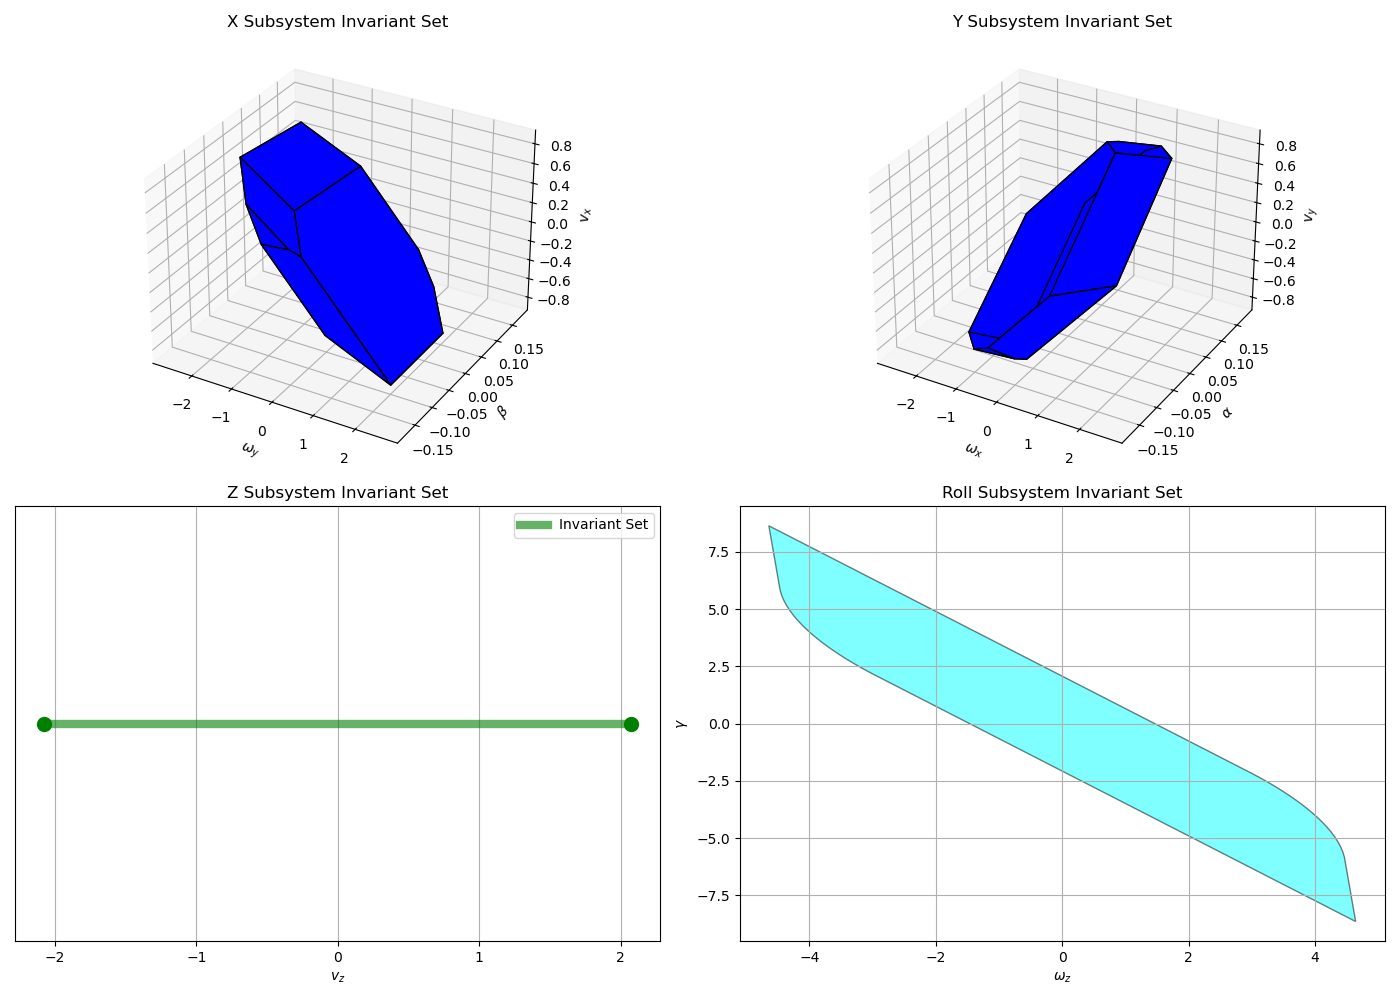
\includegraphics[width=0.9\textwidth]{figures/del3_1_sets.png}
    \caption{Maximum Output Admissible Sets (Terminal Invariant Sets) for the X, Y, Z, and Roll subsystems.}
    \label{fig:3_1_sets}
\end{figure}

\subsection*{4. Simulation Results}

The plots below show the closed-loop trajectory for the requested maneuver (starting at 5 m/s for x, y, z and 30 deg for roll). The controller successfully stabilizes the system to the origin within the required time.

\begin{figure}[H]
    \centering
    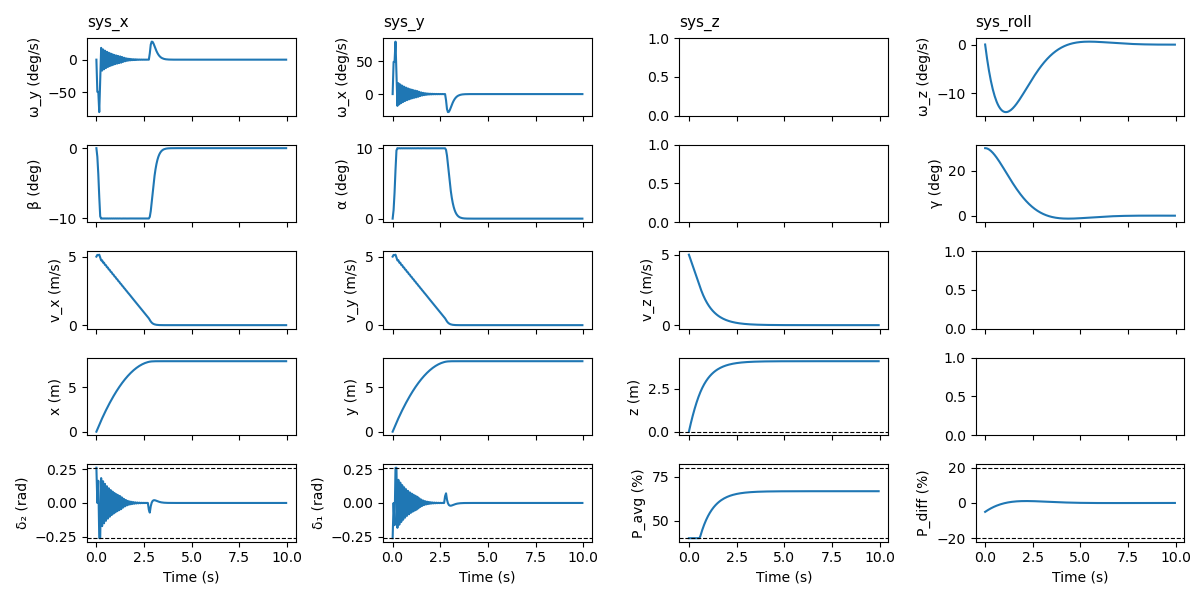
\includegraphics[width=0.9\textwidth]{figures/del3_1_sim.png}
    \caption{Closed-loop regulation results starting from non-zero initial conditions. All states converge to the origin.}
    \label{fig:3_1_sim}
\end{figure}

\section*{Deliverable 3.2: MPC Tracking}

\subsection*{1. Design Procedure}

To enable tracking of non-zero references, we modified the MPC formulation to minimize the error between the state and the reference, rather than regulating to the origin.

\begin{enumerate}
    \item  \textbf{Cost Function}: The cost function was updated to: $J = \sum_{k=0}^{N-1} ((x_k - x_{ref})^T Q (x_k - x_{ref}) + (u_k - u_{ref})^T R (u_k - u_{ref})) + (x_N - x_{ref})^T P (x_N - x_{ref})$.
        \begin{itemize}
            \item   $x_{ref}$ is the target state vector.
            \item   $u_{ref}$ is the input required to maintain the reference state (assumed $u_{ref} \approx u_s$ for velocity tracking).
        \end{itemize}
    \item  \textbf{Implementation}: We introduced a parameter \texttt{x\_ref} in the optimization problem which is updated at each step.
    \item  \textbf{Terminal Set for Tracking}: We enforced the terminal invariant set constraint for the tracking problem by shifting the set: $x_N - x_{ref} \in \mathcal{X}_f$. This ensures that if the system reaches the terminal state, it can remain within the invariant set around the reference indefinitely.
\end{enumerate}

\subsection*{2. Tuning Parameters}

We used the same tuning parameters as in Deliverable 3.1 ($H=2.0s$, same $Q$ and $R$ matrices), as they provided good performance for regulation and proved suitable for tracking as well.

\subsection*{3. Simulation Results}

The plots below show the rocket starting from the origin and successfully tracking the reference velocities ($v_x=3, v_y=3, v_z=3$ m/s) and roll angle ($\gamma=35^\circ$). The settling time is well within the 7-second requirement.

\begin{figure}[H]
    \centering
    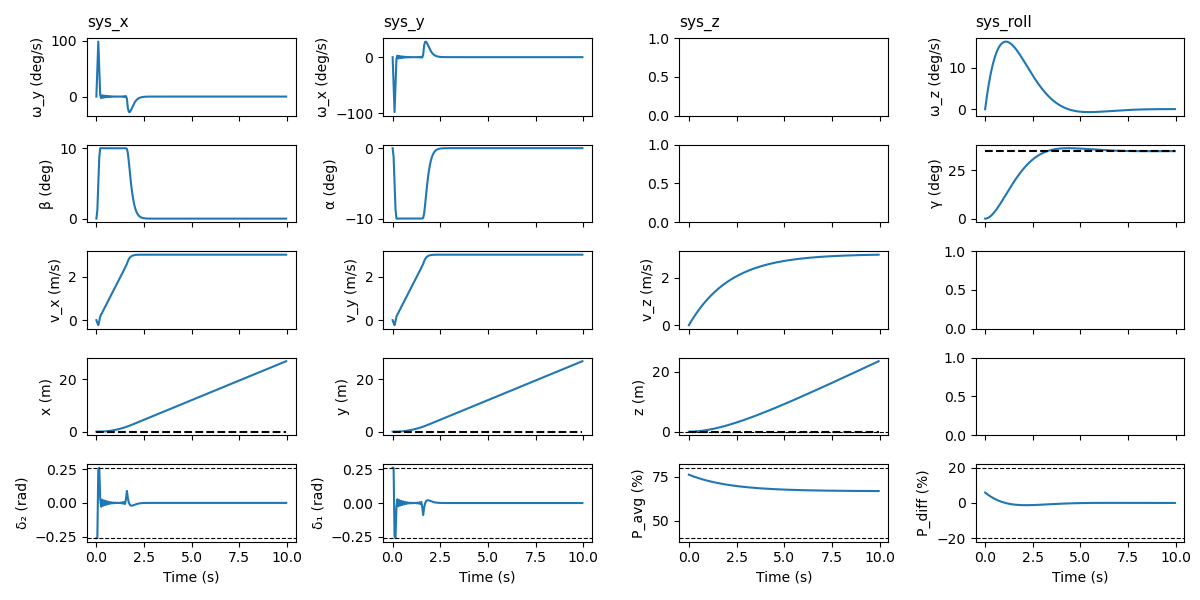
\includegraphics[width=0.9\textwidth]{figures/del3_2_sim.png}
    \caption{Closed-loop tracking results. The system tracks the constant velocity and angle references with zero steady-state error.}
    \label{fig:3_2_sim}
\end{figure}

\section*{Deliverable 3.3: Position Control (PI + MPC)}

\subsection*{1. Design Procedure}

The control objective is to take the rocket from a starting position to a stationary target point. To achieve this, we implemented a cascaded control architecture:

\begin{enumerate}
    \item   \textbf{Outer Loop (PI Position Controller)}: This controller computes the desired velocity reference ($v_{ref}$) based on the position error ($p_{ref} - p$).
    \[ v_{ref, k} = K_p (p_{ref} - p_k) + K_i \sum_{j=0}^k (p_{ref} - p_j) \cdot T_s \]
    The output of this controller is saturated to ensure physical feasibility.
    
    \item   \textbf{Inner Loop (MPC Velocity Controller)}: This is the MPC controller designed in Deliverable 3.2. It receives the $v_{ref}$ from the PI controller and computes the optimal control inputs to track this velocity.
\end{enumerate}

This separation allows us to use the MPC for fast dynamics (velocity/attitude) while handling the slower position dynamics with a simple PI controller.

\subsection*{2. Tuning Parameters}

\begin{itemize}
    \item   \textbf{MPC}: We increased the horizon to $H=5.0s$ to allow for smoother planning over longer trajectories. The weights $Q$ and $R$ remained the same as in 3.1/3.2.
\end{itemize}

\subsection*{3. Simulation Results}

The simulation shows the rocket starting at position $(50, 50, 100)$m and navigating to the target $(0, 0, 10)$m. The PI controller generates velocity references that guide the rocket to the target, and the MPC successfully tracks these references while satisfying constraints.

\begin{figure}[H]
    \centering
    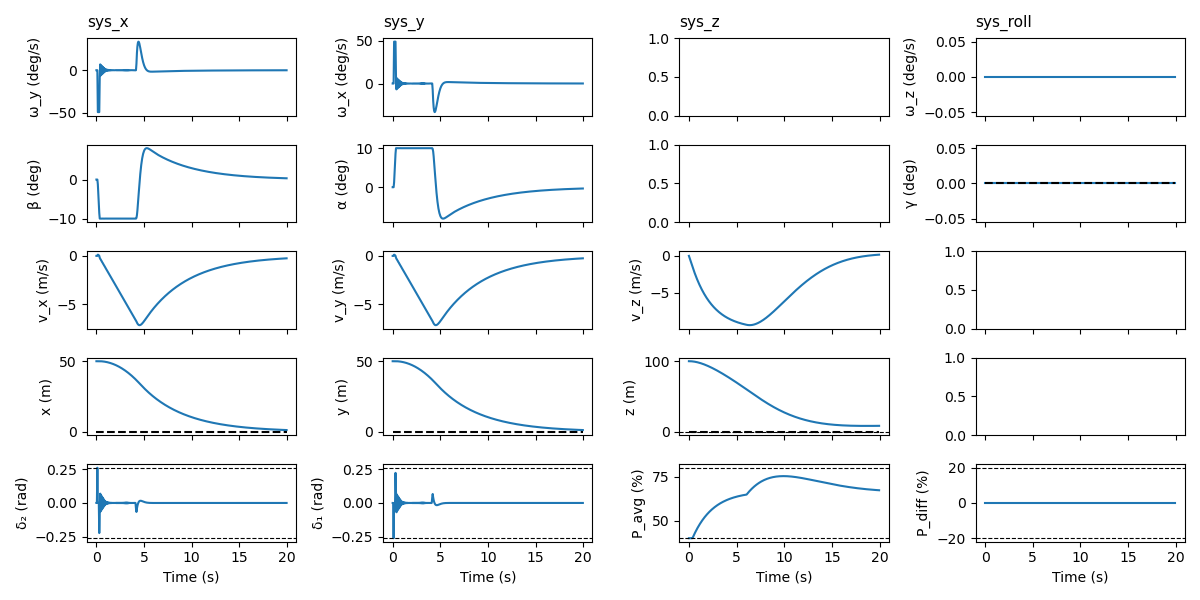
\includegraphics[width=0.9\textwidth]{figures/del3_3_sim.png}
    \caption{Closed-loop position control. The rocket successfully navigates from the initial position to the target.}
    \label{fig:3_3_sim}
\end{figure}

\section*{Deliverable 4.1: Nonlinear Simulation}

To validate the robustness of our linear controller design, we tested the controller developed in Part 3.3 (Cascaded PI + MPC) on the full \textbf{nonlinear} rocket model.

\subsection*{1. Simulation Setup}
The simulation setup is identical to Deliverable 3.3:
\begin{itemize}
    \item   \textbf{Initial Position}: $(50, 50, 100)$m.
    \item   \textbf{Target}: $(0, 0, 10)$m.
    \item   \textbf{Controller}: The same linear MPC formulation (linearized around hover) + PI position controller.
    \item   \textbf{Soft Constraints}: To ensure continuous feasibility despite the mismatch between the linear prediction model and the nonlinear plant, we enabled \textbf{soft constraints} for the state limits. We implemented an $L_1$-norm exact penalty method by introducing non-negative slack variables $\epsilon_k \in \mathbb{R}^{n_x}$ in the optimization problem. The state constraints were relaxed to $x_{min} - \epsilon_k \le x_k \le x_{max} + \epsilon_k$, and a high linear penalty term ($10^5 \cdot \sum \|\epsilon_k\|_1$) was added to the cost function. This allows for minor transient violations of the state constraints (e.g., tilt angles) rather than causing the solver to fail.
\end{itemize}

\subsection*{2. Results and Discussion}

As expected, the controller successfully guides the nonlinear system to the target. The behavior is nearly identical to the linear simulation. This indicates that:
\begin{enumerate}
    \item   The linearization around the hover point ($v=0, \theta=0$) is a valid approximation for the maneuvers performed.
    \item   The controller is robust enough to handle the small nonlinearities (e.g., Coriolis terms, trigonometric nonlinearities in rotation matrices) that are neglected in the linear model.
\end{enumerate}

\begin{figure}[H]
    \centering
    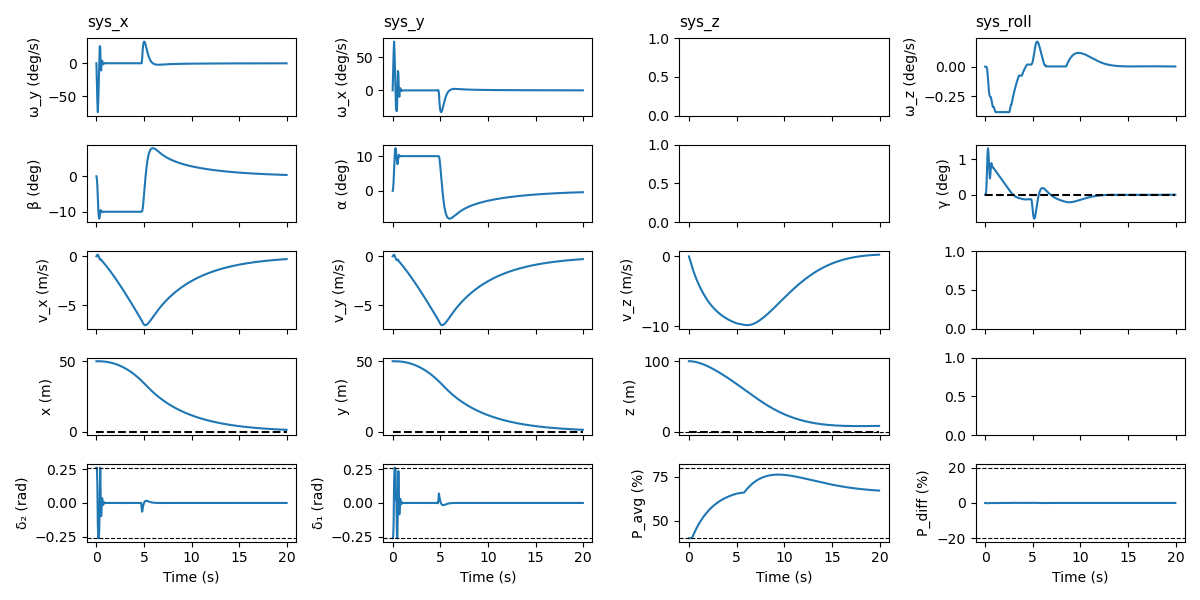
\includegraphics[width=0.9\textwidth]{figures/del4_1_sim.png}
    \caption{Result of applying the linear MPC controller to the full nonlinear system.}
    \label{fig:4_1_sim}
\end{figure}

\section*{Deliverable 5.1: Offset-Free Tracking}

\subsection*{1. Problem Identification: Baseline Tracking Failure}

In this section, we analyze the performance of the standard MPC controller when there is a significant discrepancy between the nominal model used for prediction and the actual plant. Specifically, we simulated the rocket with a mass of $1.5$ kg (with zero fuel consumption rate), while the controller assumes a nominal mass of $1.0$ kg.

As seen in Figure \ref{fig:4_1_offset}, the controller fails to track the reference z-velocity of 0 m/s. Instead, it settles at a steady-state velocity with a significant offset. This is because the feedforward gravity compensation is calculated based on the lighter nominal mass, providing insufficient thrust. The proportional feedback from the MPC eventually balances the excess gravity, but only by maintaining a permanent error.

\begin{figure}[H]
    \centering
    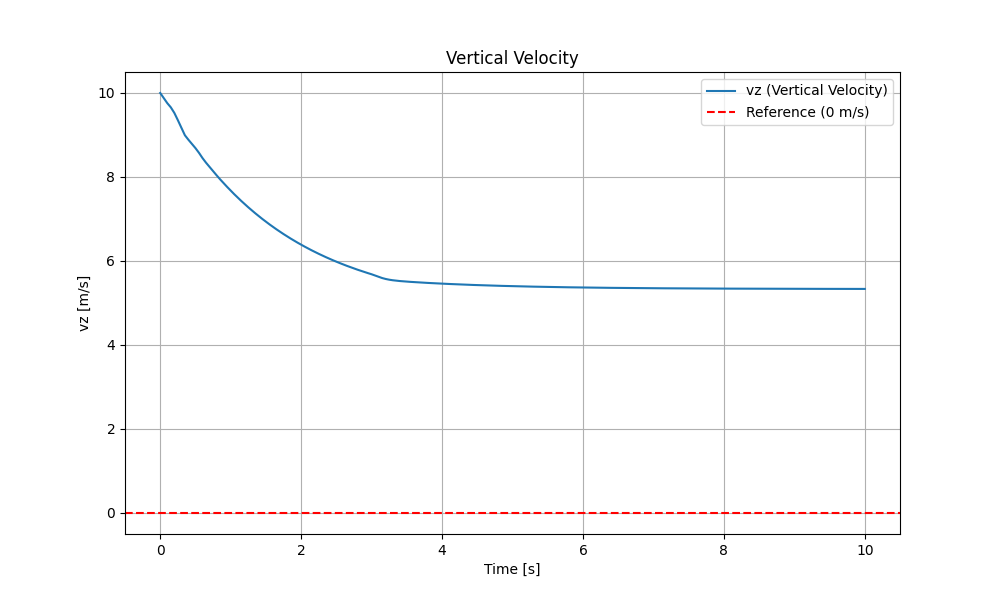
\includegraphics[width=0.9\textwidth]{figures/plot_4_1_vz_offset.png}
    \caption{Tracking performance under mass mismatch without a disturbance observer. A significant steady-state offset is observed.}
    \label{fig:4_1_offset}
\end{figure}

\subsection*{2. Solution: Disturbance Observer (DOB) Design}

To achieve offset-free tracking in the presence of model mismatch, we implemented a Disturbance Observer (DOB) based MPC.

\subsubsection*{Design Procedure}

\begin{enumerate}
    \item \textbf{Augmented State Model}:
    We augmented the system state $x$ with a constant disturbance state $d$. The augmented dynamics are:
    \begin{align*}
    x_{k+1} &= A x_k + B u_k + B_d d_k \\
    d_{k+1} &= d_k
    \end{align*}
    where $B_d$ is the disturbance input matrix. For the z-velocity subsystem, we chose $B_d = [-0.1]$ to model a disturbance affecting the vertical acceleration.

    \item \textbf{Observer Design}:
    We designed a linear observer to estimate both the state $\hat{x}$ and the disturbance $\hat{d}$ from the measurements $y_k = C x_k$. The observer dynamics are:
    \[
    \begin{bmatrix} \hat{x}_{k+1} \\ \hat{d}_{k+1} \end{bmatrix} = 
    \begin{bmatrix} A & B_d \\ 0 & I \end{bmatrix} \begin{bmatrix} \hat{x}_k \\ \hat{d}_k \end{bmatrix} + 
    \begin{bmatrix} B \\ 0 \end{bmatrix} u_k + 
    L (y_k - C \hat{x}_k)
    \]
    The observer gain matrix $L$ was computed using pole placement to ensure stable and fast convergence of the estimation error.

    \item \textbf{Disturbance Compensation}:
    The estimated disturbance $\hat{d}$ is used in two ways:
    \begin{itemize}
        \item \textbf{Target Calculation}: We adjust the target input $u_{target}$ to counteract the estimated disturbance at the steady state. We solve for $u_{target}$ such that:
        \[ (I - A) x_{ref} - B u_{target} - B_d \hat{d} = 0 \]
        \item \textbf{Prediction Model}: The MPC optimization uses the augmented model (with constant $\hat{d}$) for prediction.
    \end{itemize}
\end{enumerate}

\subsubsection*{Tuning Parameters}

\begin{itemize}
    \item \textbf{Observer Poles}: We placed the observer poles at $[0.4, 0.5]$. These are relatively fast to ensure the disturbance estimate converges quickly.
    \item \textbf{MPC Weights}: $Q = \text{diag}([100.0])$, $R = \text{diag}([0.1])$. High penalty on velocity error.
\end{itemize}

\subsection*{3. Result: Efficiency of the Correction}

With the DOB enabled, the controller successfully eliminates the steady-state error. Initially, the rocket drops due to the mass mismatch. However, the observer quickly detects the discrepancy, integrates it into $\hat{d}$, and the controller increases thrust to compensate. Since the mass mismatch creates a constant force difference in the linear model ($F_{dist} = \Delta m \cdot g$), the constant disturbance model is appropriate and estimates this force correctly once the transient dies out.

\begin{figure}[H]
    \centering
    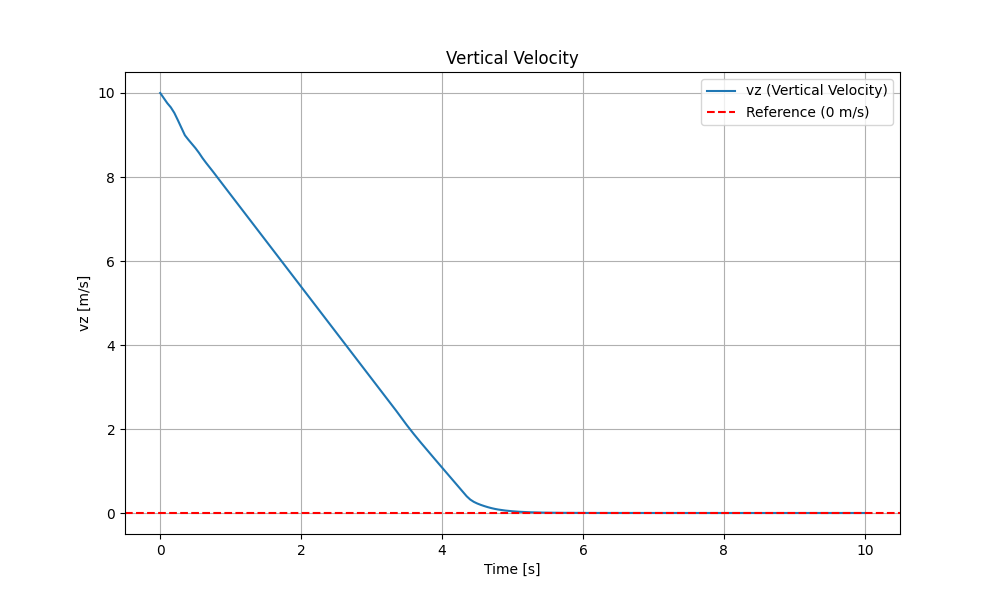
\includegraphics[width=0.9\textwidth]{figures/plot_5_1_vz_offset.png}
    \caption{Offset-free tracking with the disturbance observer. The steady-state error is eliminated.}
    \label{fig:5_1_correction}
\end{figure}

\begin{figure}[H]
    \centering
    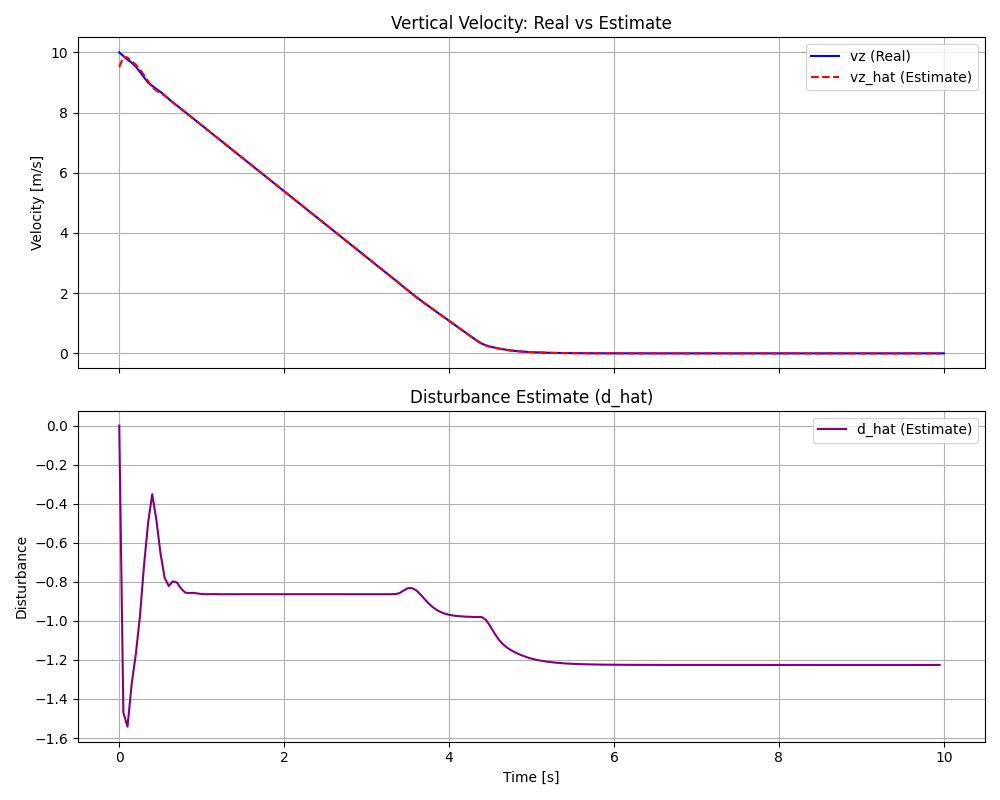
\includegraphics[width=0.9\textwidth]{figures/plot_5_1_estimates.png}
    \caption{Estimated state $\hat{v}_z$ and disturbance $\hat{d}$ converging to the true values. The disturbance estimate stabilises to compensate for the mass mismatch.}
    \label{fig:5_1_estimates}
\end{figure}

\section*{Deliverable 5.2: Time-Varying Mass}

\subsection*{1. The Time-Varying Mass Challenge}

We simulated the rocket with an initial mass of $2.0$ kg and a continuous fuel consumption rate of $0.1$ kg/s. This creates a ramp-like disturbance which allows us to test the controller against a linearly changing system parameter, violating the constant disturbance assumption ($d_{k+1} = d_k$) of our observer.

\subsection*{2. Tracking Performance Analysis}

\subsubsection*{Theoretical Limitation}
The disturbance observer assumes a piecewise constant disturbance. However, the linearly decreasing mass implies a linearly varying disturbance force (a ramp signal):
\[ F_{dist}(t) = (m(t) - m_{nom})g = (m_0 - \dot{m}t - m_{nom})g \]
According to the Internal Model Principle, an observer based on a constant disturbance model (Type 0) cannot track a ramp disturbance (Type 1) with zero error. It will inevitably exhibit a steady-state estimation error (lag).

\subsubsection*{Simulation Results}
Despite this theoretical limitation, our simulation results (Figure \ref{fig:5_2_standard}) show that the tracking offset is negligible. This is due not only to the fast observer dynamics (poles at $0.4, 0.5$) but also to our standard MPC tuning (aggressive $Q$). The high penalty on velocity error forces the controller to react strongly, keeping the lag imperceptible.

To explicitly visualize this theoretical offset, we performed a separate simulation where we intentionally "detuned" the controller by significantly reducing $Q$ (making it less aggressive), as shown in Figure \ref{fig:5_2_offset}.

\begin{figure}[H]
    \centering
    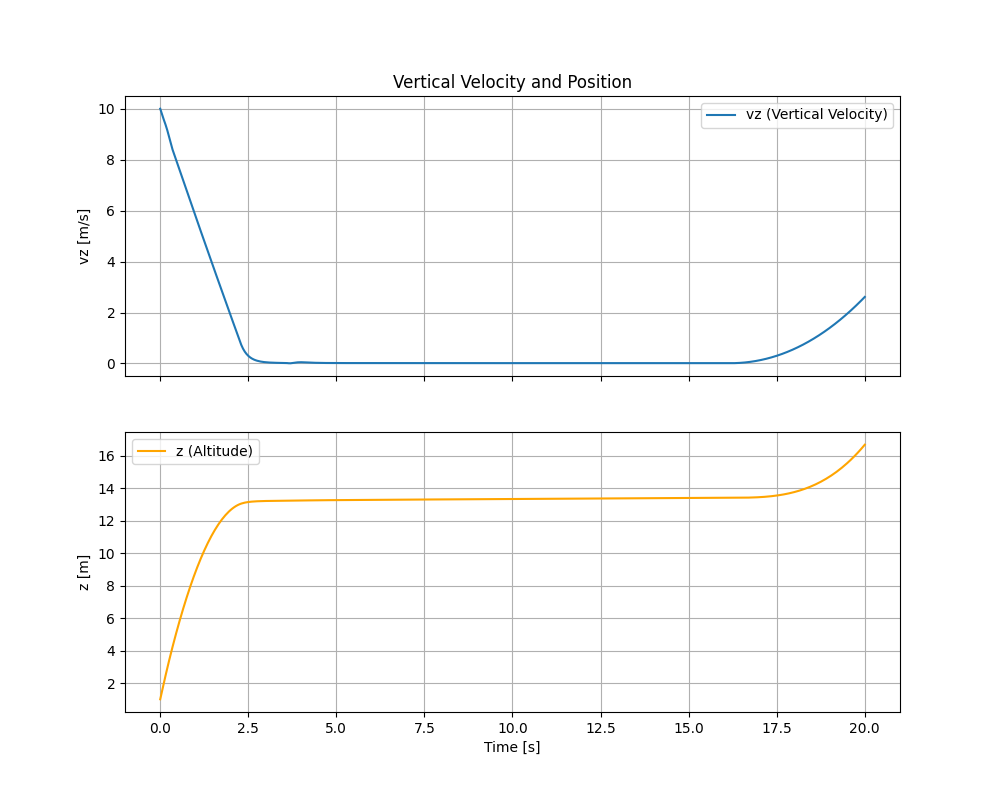
\includegraphics[width=0.9\textwidth]{figures/plot_5_2_z_vz.png}
    \caption{Tracking performance of the standard implementation (fast observer). The theoretical offset is effectively rejected.}
    \label{fig:5_2_standard}
\end{figure}

\begin{figure}[H]
    \centering
    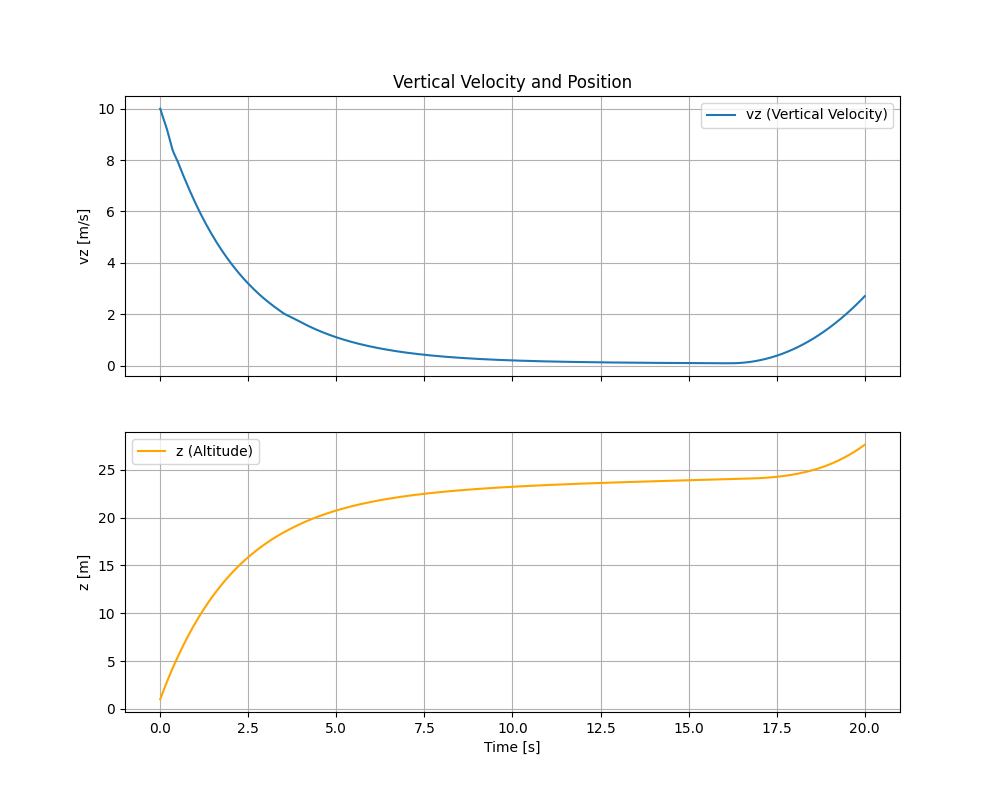
\includegraphics[width=0.8\textwidth]{figures/plot_5_2_z_vz_qrtune.png}
    \caption{Visualization of the ramp tracking lag (offset) using detuned weights to highlight the theoretical limitation.}
    \label{fig:5_2_offset}
\end{figure}

\begin{figure}[H]
    \centering
    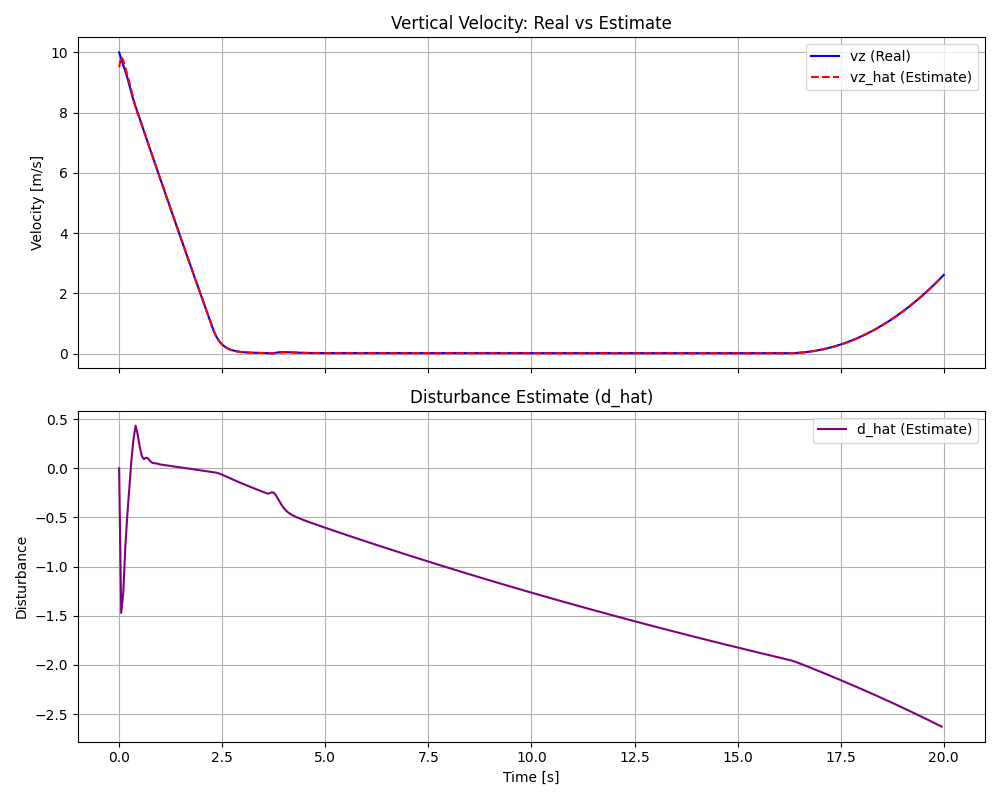
\includegraphics[width=0.8\textwidth]{figures/plot_5_2_estimates.png}
    \caption{Evolution of the estimator states. The estimated disturbance $\hat{d}$ clearly exhibits a ramp behavior (linear decrease) tracking the loss of mass, while $\hat{v}_z$ tracks the velocity.}
    \label{fig:5_2_estimates}
\end{figure}

\subsection*{3. Proposed Estimator Modification}

To achieve true offset-free tracking for a linearly changing mass, we would need to augment the disturbance model to include the \textbf{rate of change} (slope) of the disturbance:
\begin{align*}
d_{k+1} &= d_k + T_s \cdot \delta_k \\
\delta_{k+1} &= \delta_k
\end{align*}
By estimating both the disturbance $d$ and its slope $\delta$, the MPC could anticipate the future evolution.

\subsection*{4. End of Simulation Behavior}

Towards the end of the simulation, we observe an \textbf{Uncontrollable Ascent}. As fuel is consumed, the rocket becomes light enough that the thrust at the minimum constraint ($P_{avg} = 40\%$) exceeds gravity.
\[ F_{thrust, min} > m(t) \cdot g \]
Since the controller cannot lower thrust below 40\%, the rocket accelerates upwards uncontrollably.

\section*{Deliverable 6.1: Robust Tube MPC for Landing}

\subsection*{1. Robust Tube MPC Design}

To ensure a safe landing in the presence of disturbances, we implemented a Robust Tube MPC controller for the z-subsystem. The core idea is to separate the control into two parts:
\begin{enumerate}
    \item \textbf{Nominal Controller (MPC):} Computes a trajectory $z$ and input $v$ for the nominal (undisturbed) system that satisfies tightened constraints.
    \item \textbf{Ancillary Controller (Feedback):} Keeps the actual state $x$ close to the nominal state $z$ by rejecting disturbances. The control law is $u = v + K_{robust}(x - z)$.
\end{enumerate}

\subsubsection*{Separation of Controllers ($K_{robust}$ vs $K_{mpc}$)}

We explicitly separated the feedback gain used for disturbance rejection ($K_{robust}$) from the terminal cost/set gain used in the MPC optimization ($K_{mpc}$).

\begin{itemize}
    \item \textbf{$K_{robust}$ (Ancillary Controller)}:
    \begin{itemize}
        \item \textbf{Purpose}: To define the "tube" (minimal robust invariant set $E$) and keep the system inside it.
        \item \textbf{Tuning}: We chose aggressive weights ($Q_{robust} = \text{diag}([50, 200])$, $R_{robust} = 0.1$) to generate a strong feedback gain. A "stiffer" controller results in a smaller invariant set $E$, which means less tightening of the constraints is required.
    \end{itemize}
    
    \item \textbf{$K_{mpc}$ (Terminal Controller)}:
    \begin{itemize}
        \item \textbf{Purpose}: To define the terminal cost $Q_f$ and the terminal set $X_f$ for the nominal MPC problem.
        \item \textbf{Tuning}: We used weights focused on performance and stability ($Q_{mpc} = \text{diag}([10, 50])$, $R_{mpc} = 1.0$). This ensures the nominal trajectory converges smoothly to the target without being overly aggressive.
    \end{itemize}
\end{itemize}

\subsubsection*{Class Structure (\texttt{MPCControl\_base})}

We structured the code using a base class \texttt{MPCControl\_base} to handle the common MPC setup and derived classes like \texttt{MPCControl\_z} for specific subsystem logic.
\begin{itemize}
    \item \textbf{\texttt{MPCControl\_z}}: Handles the robust specific steps: computing $K_{robust}$, the invariant set $E$, the tightened constraints $\tilde{X}, \tilde{U}$, and the terminal set $\tilde{X}_f$.
    \item \textbf{\texttt{MPCControl\_base}}: Implements the generic Tube MPC optimization problem:
    \begin{itemize}
        \item Initial Constraint: $x_0 \in z_0 \oplus E$ (implemented as $E.A(x_0 - z_0) \le E.b$).
        \item Dynamics: $z_{k+1} = A z_k + B v_k$.
        \item Tightened Constraints: $z_k \in \tilde{X}$, $v_k \in \tilde{U}$.
        \item Terminal Constraint: $z_N \in \tilde{X}_f$.
    \end{itemize}
\end{itemize}

\subsection*{2. Invariant Sets and Constraints}

The key offline computations are visualized in Figure \ref{fig:6_1_sets}:
\begin{itemize}
    \item \textbf{Minimal Robust Invariant Set ($E$)}: This set bounds the error $e = x - z$. The ancillary controller ensures that if $e_0 \in E$, then $e_k \in E$ for all $k$ under bounded disturbances.
    \item \textbf{Tightened Constraints}: The nominal input constraints $\tilde{U}$ are tighter than physical limits $U$ to reserve margin for the feedback correction $K_{robust}e$.
    Specifically, the original range $40\% \le P_{avg} \le 80\%$ is reduced to ensure that $u = v + K_{robust}e$ remains feasible for all $e \in E$.
    The computed tightened set is $\tilde{U} = [-8.5637, 8.1068]$. These values represent deviations from the steady-state input $u_s \approx 56.67\%$ ($u_s$ corresponds to the trim thrust required to hover).
    Consequently, the effective input range for the nominal controller becomes:
    \[ P_{avg}^{min} \approx 56.67 - 8.56 = 48.11\%, \quad P_{avg}^{max} \approx 56.67 + 8.11 = 64.78\% \]
    This tighter range $[48.11\%, 64.78\%]$ ensures that even with the maximum expected disturbance correction added, the total thrust remains within the physical limits $[40\%, 80\%]$.
    \item \textbf{Terminal Set ($X_f$)}: The maximal invariant set for the nominal system under $K_{mpc}$, ensuring recursive feasibility.
\end{itemize}

\begin{figure}[H]
    \centering
    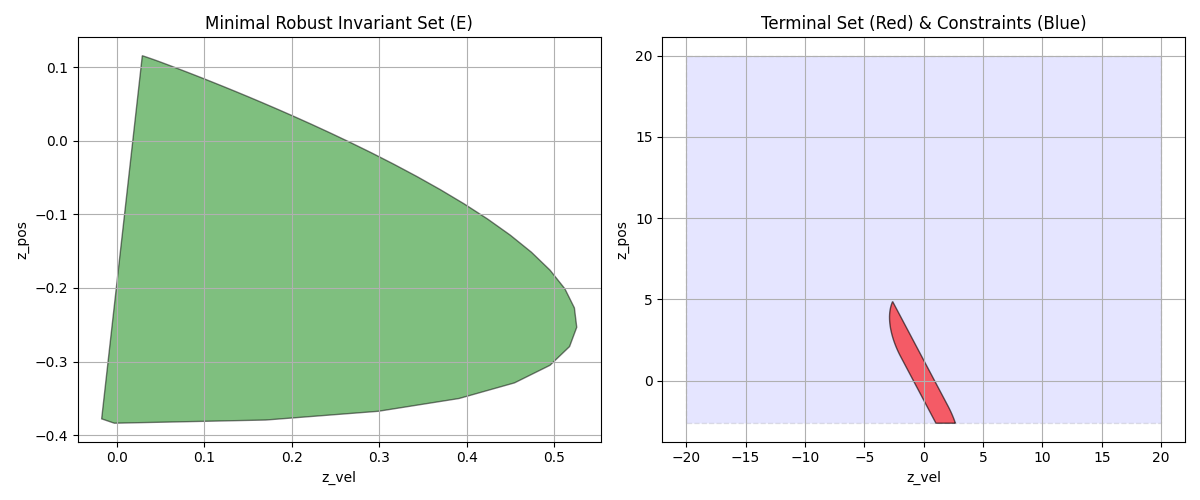
\includegraphics[width=0.9\textwidth]{figures/plot_6_1_sets.png}
    \caption{Visualisation of the Minimal Robust Invariant Set ($E$) and the Terminal Set ($X_f$) for the Robust Tube MPC.}
    \label{fig:6_1_sets}
\end{figure}

\subsection*{3. Simulation Results}

We simulated the landing maneuver from $z=10$m to $z=3$m under two disturbance scenarios:
\begin{enumerate}
    \item \textbf{Random Disturbance}: The controller successfully rejects the noise and tracks the reference. The state stays within the tube.
    \item \textbf{Extreme Disturbance}: Even with maximum disturbance, the robust controller maintains stability and constraint satisfaction (z position stays positive, input stays within bounds).
\end{enumerate}

The settling time is well within the 4-second requirement for the random disturbance case, thanks to the efficient MPC tuning. In the extreme disturbance case, the convergence is slightly slower, but this is the necessary trade-off to robustly compensate for the full range of disturbances.

\begin{figure}[H]
    \centering
    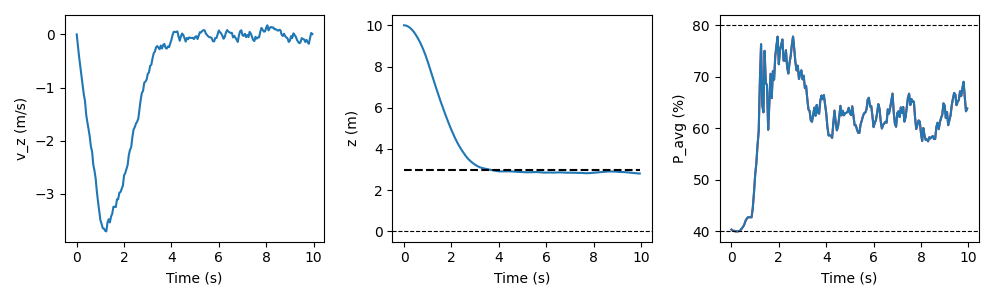
\includegraphics[width=0.9\textwidth]{figures/plot_6_1_random.png}
    \caption{Closed-loop robust MPC simulation under random wind disturbance. The robust controller keeps the system stable and tracks the reference.}
    \label{fig:6_1_sim}
\end{figure}

\begin{figure}[H]
    \centering
    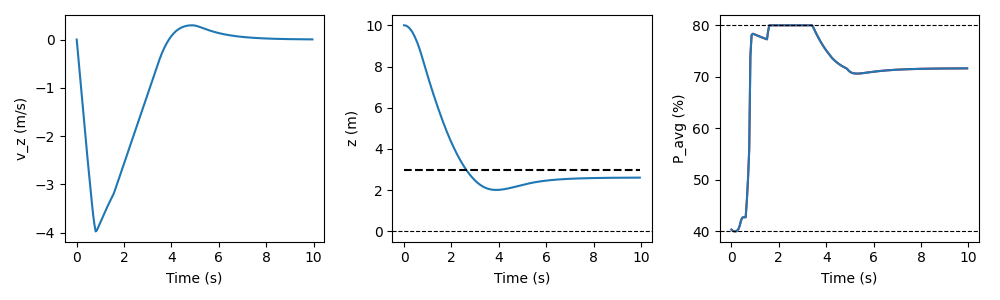
\includegraphics[width=0.9\textwidth]{figures/plot_6_1_extreme.png}
    \caption{Closed-loop robust MPC simulation under extreme disturbance. Despite the slightly slower convergence, stability and safety constraints are maintained.}
    \label{fig:6_1_extreme}
\end{figure}

\section*{Deliverable 6.2: Merged Controller for Landing}

\subsection*{1. Design Procedure}

In this part, we merged the Robust Tube MPC controller for the z-subsystem (designed in Part 6.1) with three nominal MPC controllers for the x, y, and roll subsystems. The goal is to perform a complete landing maneuver from Starting Point $(3, 2, 10)$ to Target $(1, 0, 3)$.

\subsubsection*{Controller Architecture}

We used the \texttt{MPCLandControl} class to coordinate the four independent controllers:
\begin{enumerate}
    \item \textbf{\texttt{MPCControl\_z} (Robust Tube MPC)}: Handles the vertical descent. It ensures robust constraint satisfaction ($z \ge 0$, $40\% \le P_{avg} \le 80\%$) despite disturbances.
    \item \textbf{\texttt{MPCControl\_x}, \texttt{MPCControl\_y}, \texttt{MPCControl\_roll} (Nominal MPCs)}: Handle the horizontal position and orientation. These are standard MPC controllers designed for the linearized subsystems.
\end{enumerate}

\subsubsection*{Code Structure and Reusability}

To maintain a clean codebase, the x, y, and roll controllers reuse the same \texttt{MPCControl\_base} structure as the robust controller but are configured for nominal MPC. 
\begin{itemize}
    \item \textbf{\texttt{MPCControl\_x.py}, \texttt{\_y.py}, \texttt{\_roll.py}}: These classes inherit from the base but set \texttt{self.K = 0} and \texttt{self.E = None}. This effectively disables the tube logic ($u = v$), sets the initial condition such that the first value of the planned trajectory equals the current state ($z_0 = x_0$), and enforces the standard input and state constraints.
\end{itemize}

\subsection*{2. Tuning of Nominal Controllers}

\begin{itemize}
    \item \textbf{Soft Constraints}: We enabled soft constraints for the state limits in these nominal controllers. This is crucial because the nonlinear reality might slightly violate the linear predictions, and we want to avoid infeasibility crashes in the solver.
    \item \textbf{Weights}:
    \begin{itemize}
        \item \textbf{X/Y}: $Q = \text{diag}([10, 10, 10, 50])$ (Higher weight on position to ensure convergence), $R = 1.0$.
        \item \textbf{Roll}: $Q = \text{diag}([10, 50])$, $R = 1.0$.
    \end{itemize}
\end{itemize}

\subsection*{3. Simulation Results}
\label{sec:62_sim}

The simulation demonstrates a successful landing from $(3, 2, 10)$ to $(1, 0, 3)$. The z-controller guarantees safety and robustly handles the descent, while the x/y controllers eliminate horizontal error. The rocket stabilizes within the required 4 seconds.

\begin{figure}[H]
    \centering
    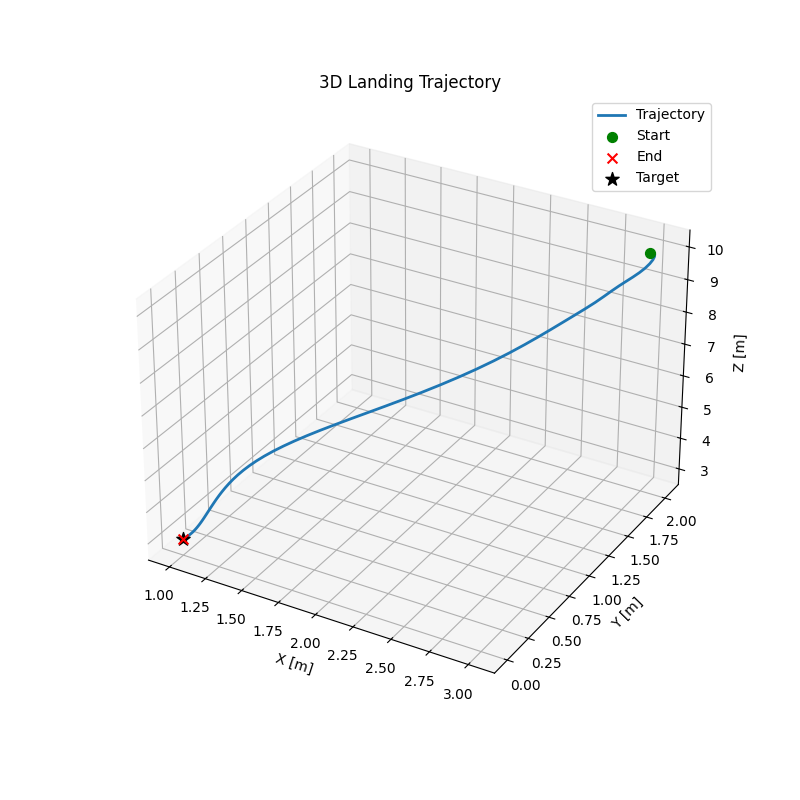
\includegraphics[width=0.8\textwidth]{figures/plot_6_2_trajectory.png}
    \caption{3D trajectory of the successful landing maneuver.}
    \label{fig:6_2_trajectory}
\end{figure}

\begin{figure}[H]
    \centering
    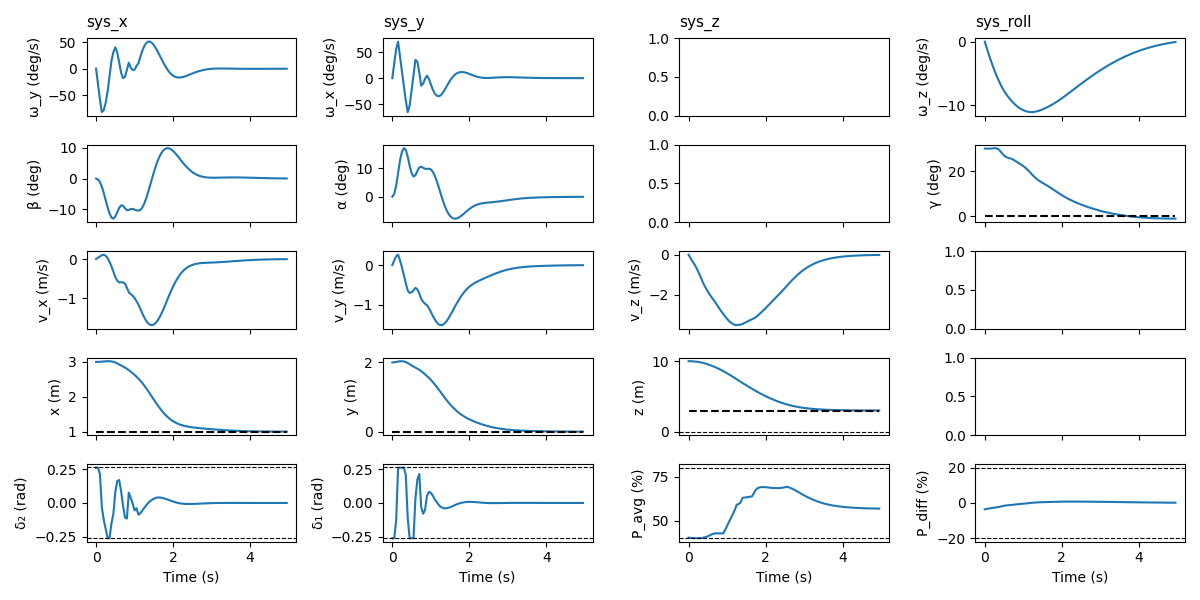
\includegraphics[width=\textwidth]{figures/plot_6_2_states.png}
    \caption{Evolution of state variables during the landing maneuver. The robust z-controller ensures constraint satisfaction while the x and y controllers drive the system to the target.}
    \label{fig:6_2_states}
\end{figure}

\section*{Deliverable 7.1: Nonlinear MPC for Landing}

\subsection*{1. Design Procedure}
In this section, we implemented a Nonlinear MPC (NMPC) controller to land the rocket. Unlike the linear MPC approaches used previously, NMPC uses the full nonlinear dynamics of the system for prediction.

\begin{enumerate}
    \item \textbf{Model}: We used the continuous-time nonlinear dynamics $\dot{x} = f(x, u)$ discretized using Runge-Kutta 4 (RK4) integration within the optimization problem.
    \item \textbf{Optimization Solver}: The problem was formulated using CasADi and solved with Ipopt, an interior-point solver for nonlinear optimization.
    \item \textbf{Cost Function}: A standard quadratic tracking cost was used:
    \[ J = \sum_{k=0}^{N-1} (x_k - x_{ref})^T Q (x_k - x_{ref}) + (u_k - u_{ref})^T R (u_k - u_{ref}) + (x_N - x_{ref})^T P (x_N - x_{ref}) \]
    \item \textbf{Terminal Cost}: The terminal weight matrix $P$ was computed by solving the DARE for the system linearized around the target state.
\end{enumerate}

\subsection*{2. Tuning Parameters}
\begin{itemize}
    \item   \textbf{Horizon}: $H = 2.0$s ($N=40$).
    \item   \textbf{Weights}:
    \begin{itemize}
        \item $Q = \text{diag}([1, 1, 1, 50, 50, 50, 10, 10, 10, 50, 50, 50])$. High penalty on angles and position to ensure precise landing.
        \item $R = \text{diag}([1, 1, 0.1, 1])$. Lower penalty on thrust ($0.1$) to allow aggressive vertical control.
    \end{itemize}
\end{itemize}

\subsection*{3. Simulation Results}
The NMPC controller successfully performs the landing maneuver from $(3, 2, 10)$ to $(1, 0, 3)$ with an initial roll of $30^\circ$. By predicting with the nonlinear model, it accurately accounts for coupling effects and trigonometric nonlinearities.

\begin{figure}[H]
    \centering
    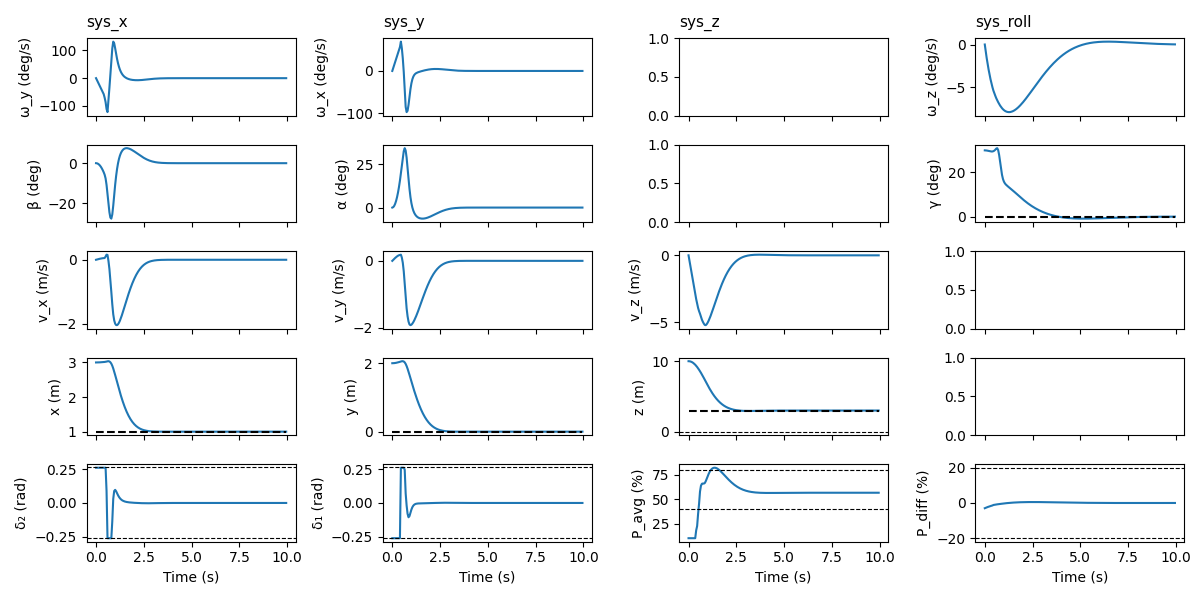
\includegraphics[width=0.9\textwidth]{figures/del7_1_sim.png}
    \caption{Landing trajectory and states using Nonlinear MPC. The controller enables a smooth landing while handling the nonlinear dynamics.}
    \label{fig:7_1_sim}
\end{figure}

\begin{figure}[H]
    \centering
    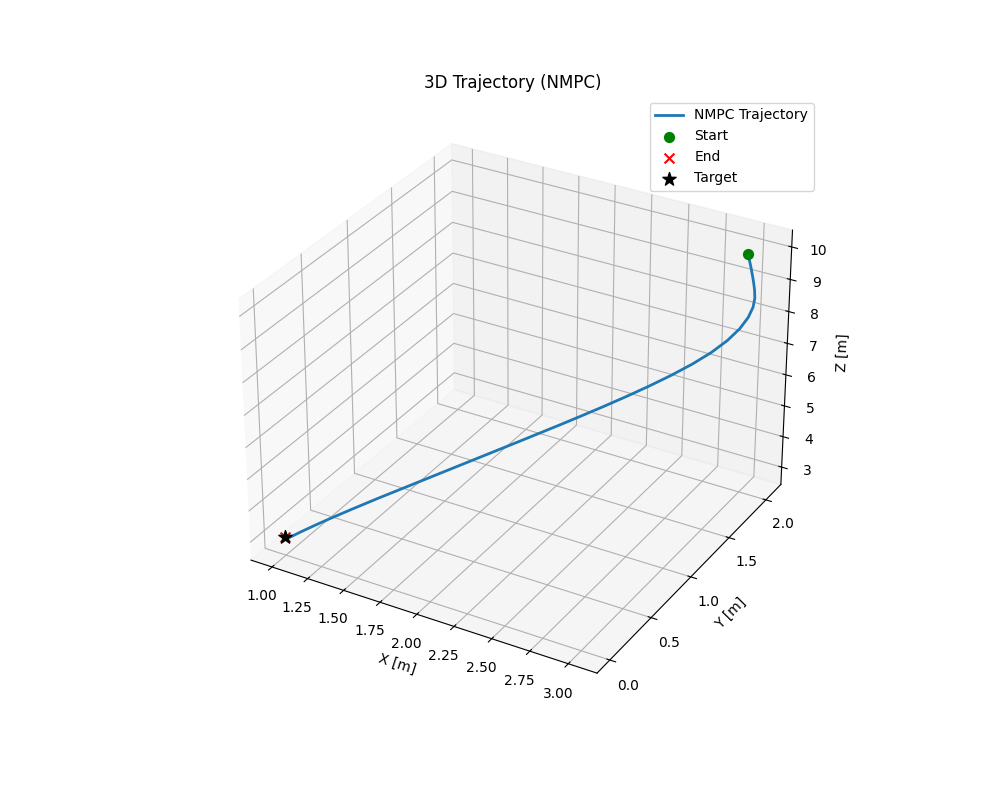
\includegraphics[width=0.8\textwidth]{figures/del7_1_trajectory.png}
    \caption{3D trajectory of the NMPC landing maneuver from $(3, 2, 10)$ to $(1, 0, 3)$.}
    \label{fig:7_1_trajectory}
\end{figure}

\end{document}
